\documentclass{beamer}

\usepackage{graphicx}

\usetheme{metropolis}           % Use metropolis theme

\title{Seed Heartbleed Lab}
\date{\today}
\author{Ward M. Zahran}
\institute{University of Jordan}
\begin{document}
  \maketitle
  \section{Prelude}

  \begin{frame}{License and Source}
  This work is licensed under CC BY-SA 4.0

  Source files and images can be found on:


  \end{frame}

  \begin{frame}{The Why}
    From RFC 6520

    ``Sending HeartbeatRequest messages allows the sender to make sure that it can reach the peer and the peer is alive.''

  \end{frame}

  \begin{frame}{The Why (cont.)}
    It is mostly ment to be used with unreliable protocols which have no session management
    to keep the connection alive without continuous data transfer.
  \end{frame}

  \begin{frame}{The How}
    The protcol consists of two types of messages:
    \begin{itemize}
     \item HeartbeatRequest
     \item HeartbeatResponse
    \end{itemize}
  \end{frame}


  \begin{frame}[fragile]{Heartbeat Message Structure}
    \begin{verbatim}
struct
{
    HeartbeatMessageType type;
    uint16 payload_length;
    opaque payload[HeartbeatMessage.payload_length];
    opaque padding[padding_length];
}
HeartbeatMessage;

    \end{verbatim}


  \end{frame}

  \begin{frame}{Heartbeat Message Structure Explained}
  \begin{itemize}
   \item

    type:  The message type, either heartbeat\_request or
    heartbeat\_response.


    \item
   payload\_length:  The length of the payload.

    \item
   payload:  The payload consists of arbitrary content.


   \item
   padding:  The padding is random content that MUST be ignored by the
   receiver.
  \end{itemize}

  \end{frame}

  \begin{frame}{The How (cont.)}

    Note that both the request and response are the same just with a differing type field value.

    A peer sends a HeartbeatRequest and then if the other peer is still alive it should echo
    back the payload in a HeartbeatResponse.

  \end{frame}

  \section{Heartbleed}
  \begin{frame}{Heartbleed Explained}
 Heartbleed is a vunrability in the OpenSSL implementation of the Heartbeat protocol.

 It results in the ability to leak an applications memory by giving a larger payload\_size
 than the actual payload in the HeartbeatRequest, the OpenSSL implementation didn't have
 bound checking code resulting in a buffer over-read vunrability, which is down to a
 memcpy() statement in the code using the unchecked payload\_length to copy from the servers
 memory into the response.

  \end{frame}

  \begin{frame}{Heartbleed Explained (cont.)}
    % Credit for image: https://en.wikipedia.org/wiki/File:Simplified_Heartbleed_explanation.svg
    % By: FenixFeather
    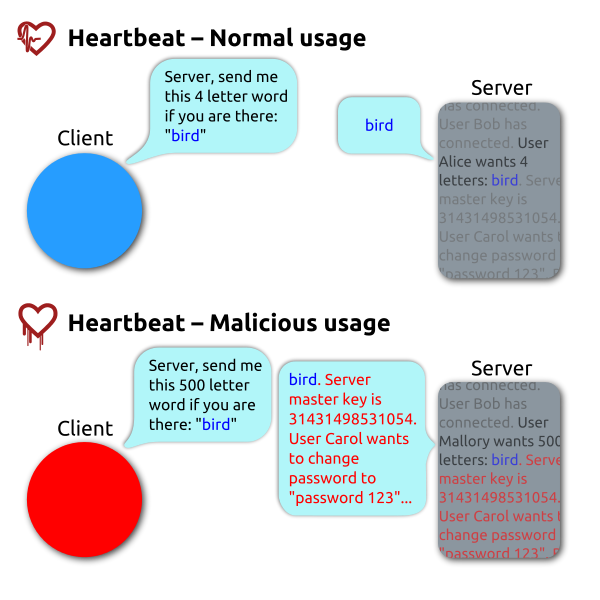
\includegraphics[width=\textheight]{heartbleed_visualization.png}
  \end{frame}

  \section{Demo}
  \begin{frame}{Demo Backround}
    The goal of this demo is to extract secrets from ELGG (a self-hosted social media)
    instance using a vunrable version of OpenSSL.

  \end{frame}

  \begin{frame}{Demo Background (cont.)}
    The first step is logging into the instance's admin account and interacting with a user
    on the victim machine machine so we have data to test on, then we run the heartbleed
    attack script on the attacker machine to leak the server memory.
  \end{frame}

  \begin{frame}{Sending A Message}
    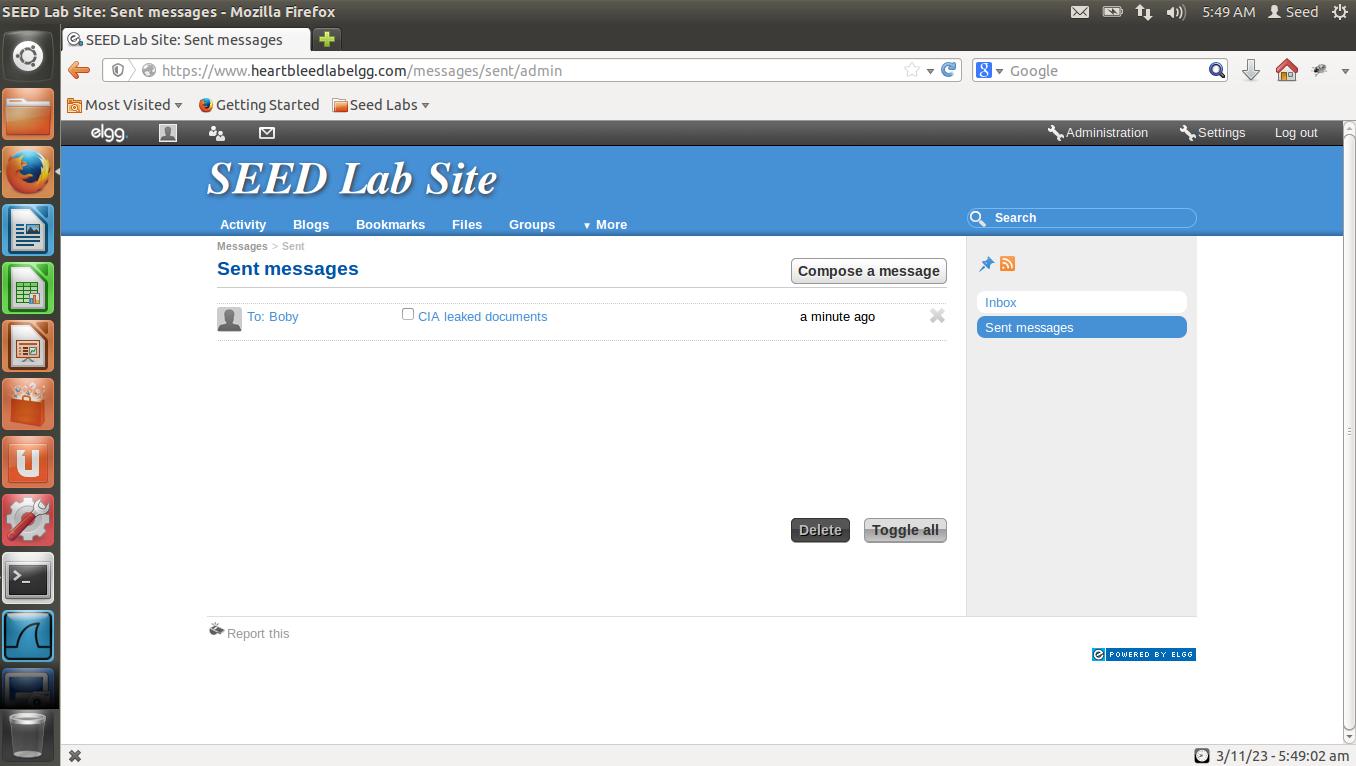
\includegraphics[width=\textwidth]{sent_message.png}
  \end{frame}

  \begin{frame}{Leaked Credentials}
    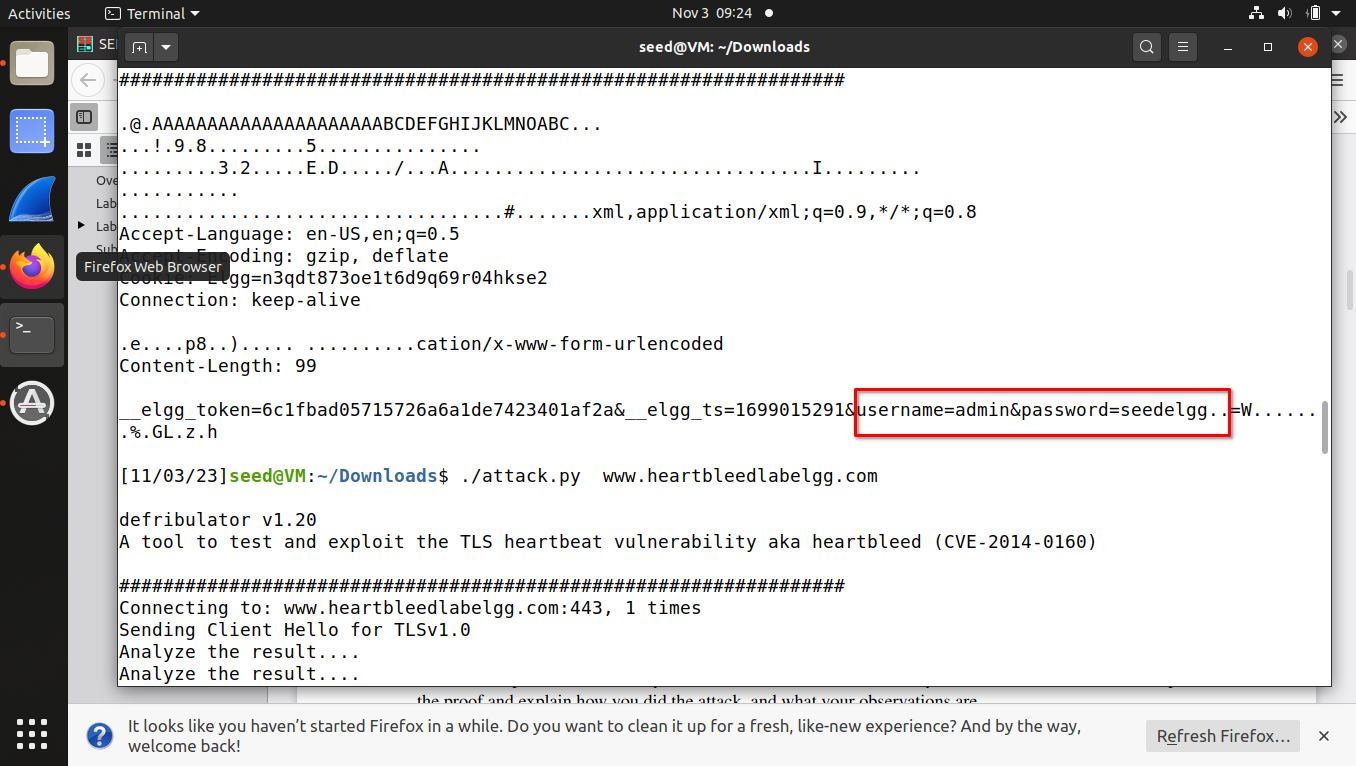
\includegraphics[width=\textwidth]{leaked_credentials.png}
  \end{frame}

  \begin{frame}{Logging to Account from the Attacker}
    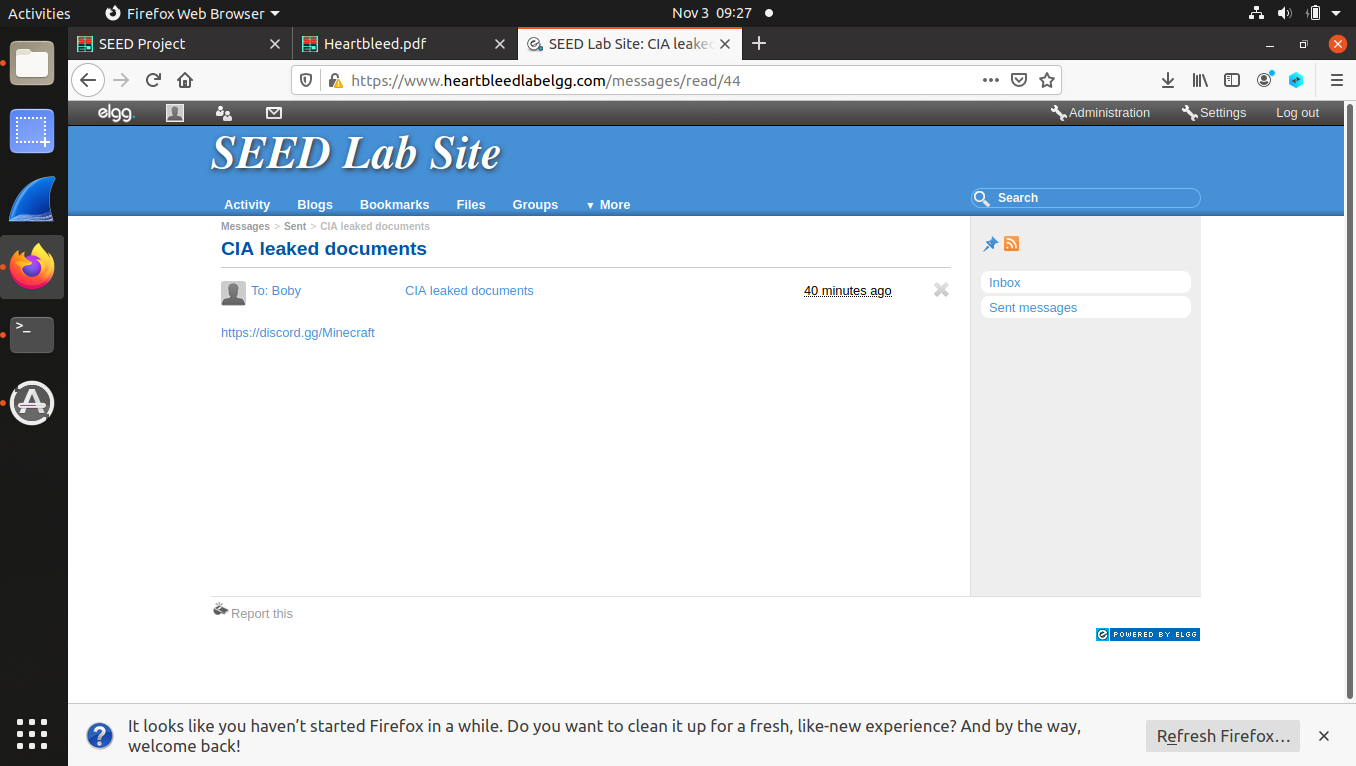
\includegraphics[width=\textwidth]{attacker_sent_message.png}
  \end{frame}

  \begin{frame}{Countermeasures}
    The Heartbleed vunrability can be patched by updating to version 1.0.1g or newer of
    OpenSSL.
  \end{frame}

  \section{Misc.}
  \begin{frame}{payload\_length and Its Effect}
  \begin{itemize}
   \item
    The payload length is an unsigned 16 bit integer meaning we have a range of 0 - 65535
    to select from, but using a payload\_length of 22 or lower he Heartbeat query will
    receive a response packet without attaching any extra data making it benign.
   \item
   Obviously the side effect of increasing the payload\_length will result in more data
   sent back to the attacker.
  \end{itemize}
  \end{frame}

  \begin{frame}{Heartbeat payload\_length Boundry}
    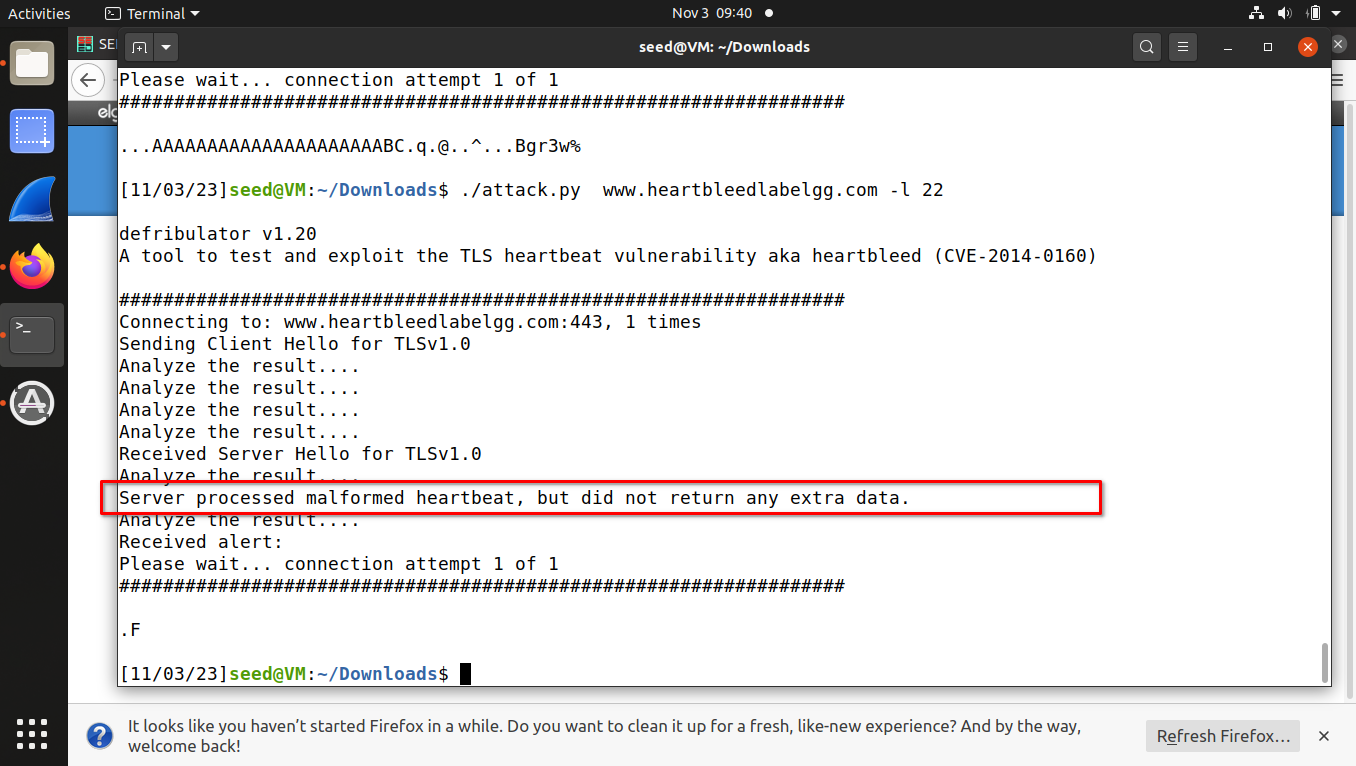
\includegraphics[width=\textwidth]{heartbleed_boundry.png}
  \end{frame}

  \begin{frame}
  Thanks for listening.
  \end{frame}
\end{document}
